It is without doubt that our understanding of how to build reliable systems out of unreliable components has led the development of robust and fairly reliable large-scale software and networking systems. The inherent instability of extreme-scale distributed systems of the future in terms of the envisioned high-rate and diversity of faults, however, calls for a reconsideration of the fault tolerance problem as a whole. % and the exploration of radically different approaches that go beyond adapting or optimizing well known and proven techniques.

Shadow Replication is a computational model that goes beyond adapting or optimizing well known and proven techniques, and explores radically different methodologies to fault tolerance~\cite{mills_2014_icnc,mills_2014_pdp,mills2014power}. % that scale to extreme-scale computing infrastructures. 
The proposed solutions differ in the type of faults they manage, their design, and the fault tolerance protocols they use. It is not just a scale up of  ``point" solutions, but an exploration of innovative and scalable fault tolerance frameworks. 
When integrated, it will lead to efficient solutions for a ``tunable" resiliency that takes into consideration the nature and requirements of the application.

The basic tenet of Shadow Replication is to associate with each main process a suite of “shadows” whose size depends on the 
``criticality" of the application and its performance requirements. Each shadow process is an exact replica of the original 
main process, 
and a consistency protocol assures that each shadow process stays consistent with its associated main process.  
Shadow Replication achieves power awareness under QoS requirements by dynamically adjusting the execution rates in response to failures. 
To save power, the shadows initially execute at a lower rate than the main process.
If the main process completes the task successfully, the associated shadows will be terminated immediately. If the main process fails, however, one of the shadow processes will be promoted to a new main process, and possibly increases its execution rate to mitigate delay.

Since the individual failure rate is extremely low, in most instances the main process will not encounter any failure and complete the task. 
Consequently, the additional energy consumed by the
slower shadow is significantly lower than that of a full-speed replica of the
main, resulting in a lot of energy savings. Furthermore, a failure of a shadow process has no bearing on the behavior of its associated main process. These two properties make it possible for Shadow Replication to enable fault tolerance at a much lower cost.

\section{Execution Model}
%Assuming the fail-stop fault model, where a processor stops execution once a fault occurs and failure can be detected by other processors~\cite{gartner_faults_1999,cristian_comm_1991}, 
Assuming there is a Reliability Availability and Serviceability (RAS) system for fault detection~\cite{ferreira_sc_2011}, 
the Shadow Replication fault-tolerance model is formally defined as follows:
\begin{itemize}
	\item A main process, $P_m(W,\text{ }\sigma_m)$, whose responsibility is to executes a task of $W$ workload at an execution rate of $\sigma_m$;
	\item A suite of shadow processes, $P_{s}(W,\text{ }\sigma_b^s, \text{ }\sigma_a^s)$ ($1 \le s \le \cal S)$, where $\cal S$ is the size of the suite. The shadows execute on separate computing nodes. Each shadow process is associated with two execution rates. All shadows start execution simultaneously with the main process at rate $\sigma_b^s$ ($1 \le s \le \cal S$). Upon failure of the main process, all shadows switch their executions to $\sigma_a^s$, with one shadow being designated as the new main process. This process continues until completion of the task.
\end{itemize}

%Assuming a single process failure, Figure \ref{fig:sc_overview} illustrates the behavior of Shadow Replication with one shadow per task. 
To illustrate the behavior of Shadow Replication, we limit the number of shadows to a single process and consider the scenarios depicted in Figure \ref{fig:sc_overview}, assuming a single process failure. 
%If the main process does not fail, it will complete the task ahead of its shadow at $t_c^m$. At this time, we terminate the shadow immediately to save energy. If the shadow fails before the main completes, the failure has no impact on the progress of the main. If the main fails, however, the shadow switches to a higher speed and completes the task at time $t_c^s$. 
Figure \ref{fig:sc_no_fail} represents the case where neither the main nor the shadow fails. The main process, executing
at a higher rate, completes the task at time $t_c^m$. At this time, the shadow process, progressing at a lower rate, stops execution immediately to save energy. Figure \ref{fig:sc_shadow_fail} represents the case where the shadow experiences a failure. This failure, however, has no impact on the progress of the main process, which still completes the task at $t_c^m$. Figure \ref{fig:sc_main_fail} depicts the case where the main process fails while the shadow is in progress. After detecting the failure of the main process, the shadow begins execution at a higher rate, completing the task at time $t_c^s$. 
%Given that the failure rate of an individual node is much lower than
%the aggregate system failure, it is very likely that the main process
%will always complete its execution successfully, thereby achieving fault tolerance at a significantly reduced cost of energy consumed by the shadow. %saving a lot of energy for its associated shadow processes. 

\afterpage{
\begin{figure}[!h]
	\begin{center}
		\subfigure[No Failure]
		{
			\label{fig:sc_no_fail}
			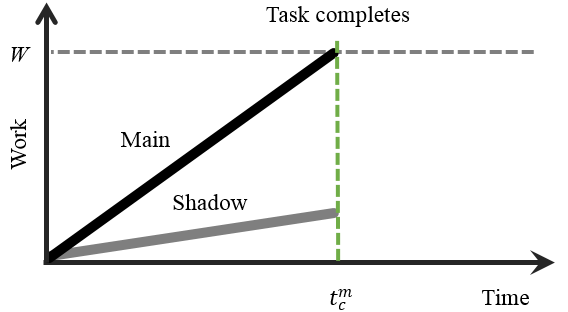
\includegraphics[width=0.6\textwidth]{Figures/exe_dy_1}
		}
		\subfigure[Shadow Process Failure]
		{
			\label{fig:sc_shadow_fail}
			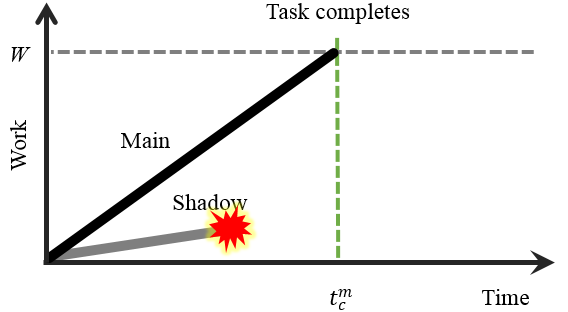
\includegraphics[width=0.6\textwidth]{Figures/exe_dy_2}
		}
		\subfigure[Main Process Failure]
		{
			\label{fig:sc_main_fail}
			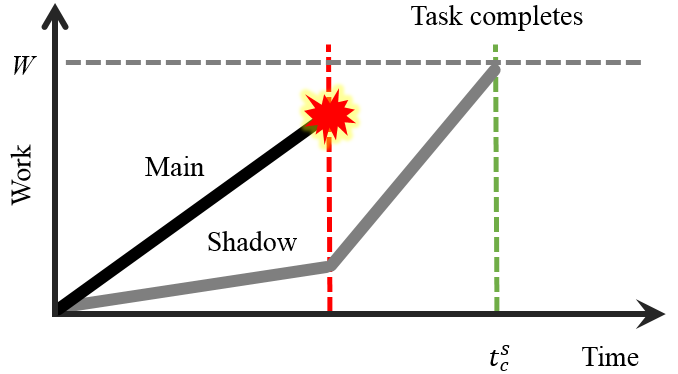
\includegraphics[width=0.6\textwidth]{Figures/exe_dy_3}
		}
	\end{center}
	\caption{Shadow Replication for a single task using a pair of main and shadow.}
	\label{fig:sc_overview}
\end{figure}
\clearpage
}



\section{Adaptivity}
\label{sec:shadowing_adaptivity}
In HPC and Cloud systems, performance, resilience, and power consumption are more often than not conflicting objectives. For example, achieving fault tolerance comes with a cost of redundant resources, which unavoidably lead to additional power and energy consumption. 
On the other hand, it has been shown that lowering supply voltages, a commonly used technique to conserve power, increases the probability of transient faults~\cite{chandra2008defect,zhao2008reliability}, and introduces non-trivial performance degradation~\cite{wang2013impact}.

Shadow Replication is a pioneering work in exploring the trade-offs among failure-free operation, the imposed power constraints, and the time to solution of the supported application. 
Internally, Shadow Replication has a set of parameters,    lying on two dimensions, that collectively determine its behavior along with costs. By configuring the shadow suite size based on fault tolerance needs, and dynamically adjusting the main and shadow processes' execution rates, Shadow Replication is able to guarantee a specific performance with certain fault tolerance capability and under a bounded power budget, thereby achieving adaptivity to the desired balance among the three conflicting objectives. 

The size of shadow suite directly reflects the amount of redundancy needed. The more shadows in each suite, the more hardware resources are required to execute the replicas in parallel. Furthermore, the additional hardware resources place a higher demand on the power supply. Therefore, it is desirable to use as few shadows as possible, under the premise that the resilience requirements are met. It is well known that one can use $f+1$ replicas to tolerate $f$ crash failures, and use $2f+1$ replicas to correct $f$ silent failures. To deal with one crash failure, a single shadow that runs as a slower replica of its associated main would be sufficient to maintain acceptable response time. Like shown in Figure~\ref{fig:sc_overview}, two replicas guarantee that at least one can complete the task, if at most one crash failure could occur. Similarly, two shadows are sufficient to guard a main process against a silent failure. Specifically, by using a simple voting mechanism and comparing the outputs of three replicas, one can detect as well as correct a silent failure~\cite{fiala_2012_sdc}. 

In addition to shadow suite size, another dimension of control consists of the execution rates of both the main and shadow processes, before and after failure. 
A closer look at the model reveals that Shadow
Replication is a generalization of traditional fault tolerance
techniques, namely re-execution and process replication. If it allows for flexible completion time, 
Shadow Replication converges to re-execution as
the shadow remains idle during the execution of the main process and
only starts execution upon failure. If the target response time is
stringent, however, Shadow Replication converges to process replication,
as the shadow must execute simultaneously with the main at the maximum
rate. Assuming dual modular redundancy to deal with a crash failure, this adaptability of Shadow Replication is further illustrated in Figure~\ref{fig:three_lines}. 
It is not difficult to imagine that by exploring the combination of execution rates, Shadow Replication covers a ``spectrum" of fault tolerance strategies, including both re-execution and process replication. 
The flexibility of the Shadow Replication model provides the
basis for the design of a fault tolerance strategy that strikes a balance between task completion time and energy saving. 

\begin{figure}[t]
	\begin{center}
		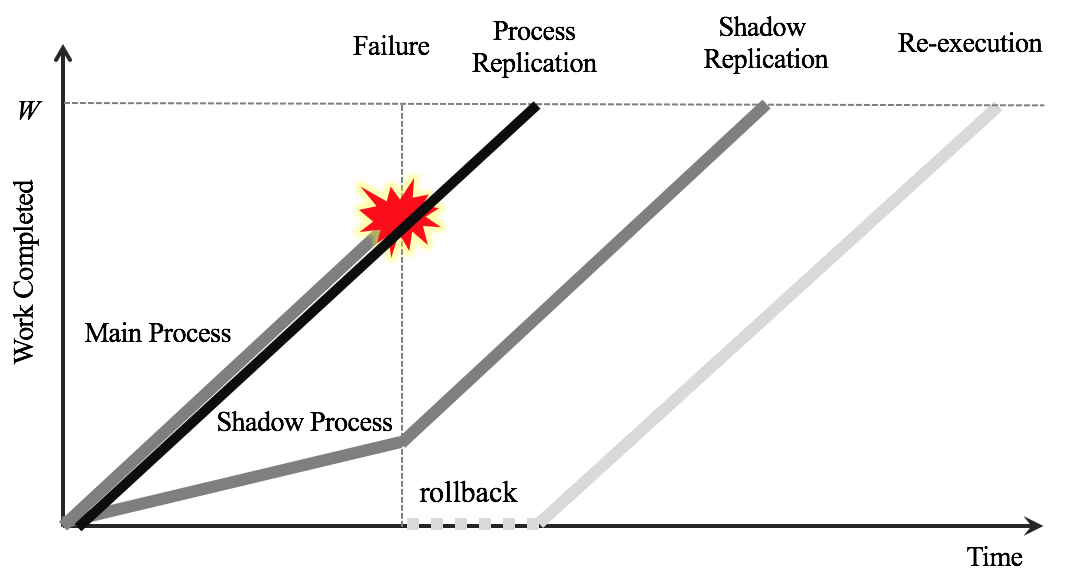
\includegraphics[width=0.8\textwidth]{Figures/three_lines}
	\end{center}
	\caption{Illustration of Shadow Replication's ability to converge to either re-execution or traditional process replication.}
	\label{fig:three_lines}
\end{figure}

\section{Execution Rate Control}

The Shadow Replication model relies on the fact that power savings can be achieved by reducing process execution rate. Furthermore, Shadow Replication needs to dynamically adjust the process execution rates to maintain satisfactory response time while saving power and energy. So far, two techniques have been explored to achieve the desired process execution rate. The first technique directly relates to a hardware feature, while the second one can be easily done via process mapping on any hardware platform.

DVFS is the first technique that our lab studied to reduce the execution rate of a process. While running each main and shadow process on a separate CPU, DVFS allows to reduce the CPU frequency by lowering the supply voltage. In the case of a failure, DVFS also allows to dynamically increase the CPU frequency to speed up a process. It is well known that one can reduce the dynamic CPU power consumption at least quadratically by reducing the frequency linearly, thereby saving power and energy simultaneously. %Its effectiveness, however, may be markedly limited by the granularity of voltage control, the range of frequencies available, and the negative effects on reliability~\cite{Eyerman:2011:FDU:1952998.1952999,zhao2008reliability,zhao2011generalized}.

An alternative approach to DVFS is to collocate multiple processes on a single CPU, while keeping each CPU running at the maximum frequency~\cite{cui_2016_scalcom}. The desired process execution rate can be achieved by controlling the \textit{collocation ratio}, which is defined as the number of processes that time-share a CPU. An example of collocation is depicted in Figure~\ref{fig:sc_mapping},  with a collocation ratio of 3 for shadow processes. A \textit{shadowed set} refers to a set of mains and their collocated shadows. The advantages and disadvantages of collocation will be further discussed in later chapters. 

\begin{figure}[t]
	\begin{center}
		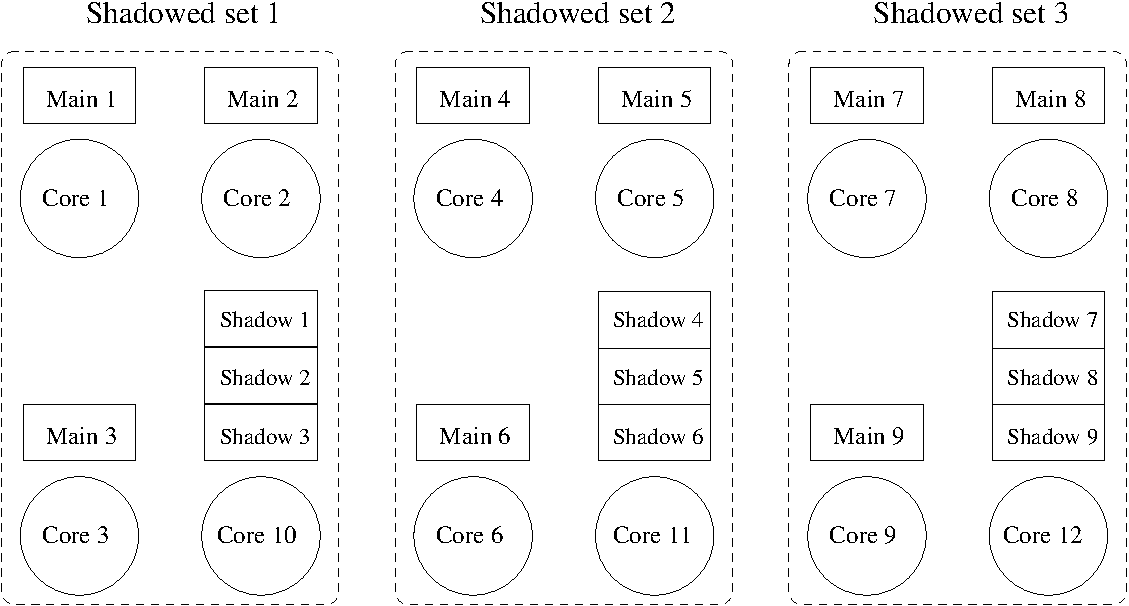
\includegraphics[width=0.8\textwidth]{Figures/sc_mapping.pdf}
	\end{center}
	\caption{An example of collocation. Nine mains and their associated shadows are grouped into three logical shadowed sets. By collocating every three shadows on a core, twelve cores are required.}
	\label{fig:sc_mapping}
\end{figure}

In terms of power and energy saving, DVFS has a different effect from collocation. 
When applying collocation, it is straightforward that fewer hardware resources are required to support the same number of processes than using DVFS. For example, only 12 cores are required to simultaneously execute 18 processes, as shown in Figure~\ref{fig:sc_mapping}. This is a 33.3\% saving in hardware resources compared to DVFS. As a result, collocation brings in reduction in power and energy consumption proportionally to the reduction in hardware resources. On the other hand, although DVFS requires the same amount of hardware as traditional process replication, it saves CPU dynamic power on each process that executes at a reduced rate, thus achieving energy savings. This thesis does not carry out a quantitative comparison between these two techniques, because the exact power and energy consumption largely depend on the specific architecture, such as the ratio between CPU dynamic power and static power, and the relationship between power reduction and frequency reduction due to DVFS.

\section{Summary}
Based on DVFS, Mills studied the Shadow Replication computational model and associated one shadow process with each main process to tolerate fail-stop failures in HPC systems. For HPC throughput consideration, his work assumes that the main process always executes at the maximum rate. Even with this restriction, Mills successfully demonstrates that Shadow Replication can achieve resilience more efficiently than both checkpoint/restart and process replication when power is limited~\cite{mills_2014_icnc,mills_2014_pdp,mills2014power}.

Although DVFS is widely available in today's processors, its effectiveness, however, may be markedly limited by the granularity of voltage control, the range of frequencies available, and the negative effects on reliability~\cite{Eyerman:2011:FDU:1952998.1952999,zhao2008reliability,zhao2011generalized}. At the same time, there are several issues with the Shadow Replication model that have been later identified and that question the applicability of Shadow Replication to tolerating high rate and diverse types of failures in extreme-scale computing environments. 
In the following chapters, this thesis presents novel work that not only addresses the limitations of the basic Shadow Replication model to achieve better adaptivity, sustainability, and scalability, but also verifies the model with prototype implementation and performance evaluation.
 



